\leadchapter{
  This chapter is a general introduction to the Hawkes processes and the challenges explored in this manuscript.
  After a succinct presentation of Hawkes processes, 
  we contextualise the state-of-the-art literature concerning estimation methods for Hawkes processes in Section~\ref{sec:chap0_introduction}. 
  This allows us to exhibit the two paradigms that are studied in this work and we present our contributions in the subsequent sections:
  Section~\ref{sec:chap0_inhibition} pertains to the parametric estimation of both univariate and multivariate Hawkes processes with eventual inhibiting interactions (Chapters~\ref{chapter:univariate_inhibition} and \ref{chapter:multivariate_inhibition}).
  Section~\ref{sec:chap0_missing_data} presents our contributions to the study of exciting Hawkes processes by accounting for certain models of imperfect data (Chapters~\ref{chapter:spectral_superposition} and \ref{chapter:spectral_thinning}).
}

\chapter{Introduction}

\section{The mathematical setting}\label{sec:chap0_introduction}
\subsection{A quick dive into Hawkes processes}\label{sec:chap0_hawkes_process}
    \begin{itemize}
        \item multivariate
        \item intensity function with non-linear, specify positive part, kernel, baseline
        \item stationarity and existence conditions
        \item parametric setting ? 
        \item log-likelihood
    \end{itemize}
\subsection{Inference methods for Hawkes processes: the state-of-the-art}\label{sec:chap0_related_works}
\begin{itemize}
    \item estimation methods
    \item parametric
    \item inhibition
    \item missing data
    \item spectral ? 
\end{itemize}

\section{Encouraging restraint: factoring in inhibition for Hawkes processes}\label{sec:chap0_inhibition}
    \subsection{Maximum Likelihood Estimation for Hawkes Processes with self-excitation or inhibition}
        Chapter~\ref{chapter:univariate_inhibition} focuses on the univariate Hawkes process $N$ on $\RR_{\geq0}$, where the conditional intensity function reads, for any $t>0$:
        \[\lambda(t) = \left(\mu + \int_{0}^{t}{h(t-s)\,N(\dd s)}\right)+ = \left(\mu + \sum_{k=1}^{N(t)}{h(t - T_k)}\right)^+\,,\]
        where $\mu > 0$ and $h\colon \RR_{\geq 0} \to \RR$ is a monotone function such that $\|h\|_1 < 1$. 
        By allowing $h$ to be either a positive or a negative function, this model covers both self-exciting and self-inhibiting settings.

        The main contribution in this framework is to propose a parametric estimation method of intensity $\lambda$ through maximum likelihood estimation. 
        The maximum likelihood estimator for self-exciting Hawkes processes was previously established in \textcite{Ozaki1979} but is unable to properly take into account eventual inhibiting effects. 
        In order to adapt the procedure to our context, it is necessary to compute explicitely both the conditional intensity function and the compensator $\Lambda$ defined as:
        \[\Lambda(t) = \int_{0}^{t}{\lambda(s)\,\dd s}\,,\]
        for all $t>0$

        To carry out this study, we first introduce the \textit{underlying intensity function} of $N$, noted $\lambda^\star$ and defined, for any $t>0$, as:
        \[\lambda^\star(t) = \mu + \int_{0}^{t}{h(t-s)\,N(\dd s)}\,.\]
        The advantage of studying $\lambda^\star$ is that, between any two consecutive event times $T_{k-1}$ and $T_k$, $\lambda^\star$ inherits properties such as smoothness and strict monotony from the interaction function $h$.
        Furthermore, recovering $\lambda$ is immediate as it suffices to notice that $\lambda(t) = \left(\lambda^\star(t)\right)^+$, for all $t>0$. 

        The underlying intensity function is a means to an end, as it allows us to introduce the \textit{restart times} $T_k^\star$, for any integer $k$, defined as:
        \[T_k^\star = \inf{\{t\geq T_i\mid \forall t\in(T_k^*,T_{k+1}),\, \lambda(t) = \lambda^\star(t)\}}\,.\]

        \begin{figure}[!ht]
            \centering
            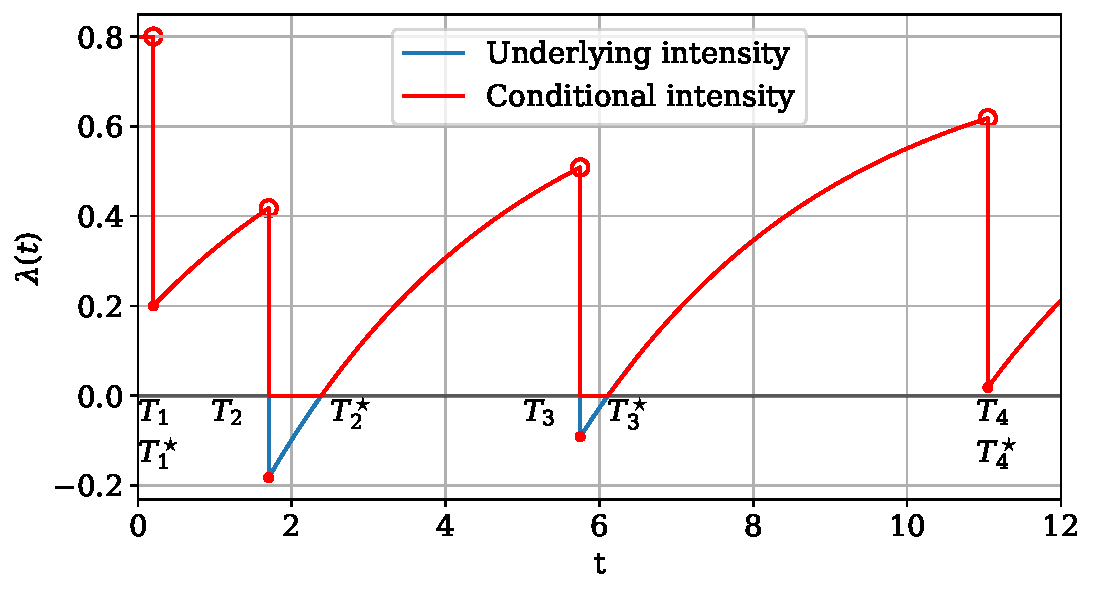
\includegraphics[width=0.6\textwidth]{images/chapter2/cooldownTimesMarkedSerif2.pdf}
            \caption{}
            \label{fig:chap0_univariate_underlying_examples}
        \end{figure}



    \subsection{Inference of multivariate exponential Hawkes processes with inhibition and application to neuronal activity}
\section{Something is amiss: how to account for missing data?}\label{sec:chap0_missing_data}
    \subsection{Spectral analysis for the  inference of noisy Hawkes processes}
    \subsection{A numerical exploration of thinned Hawkes processes through spectral theory}
    Inference results including estimation and goodness-of-fit/testing.

    
    \section*{Outline of the manuscript} The chapters in this manuscript are independent from each other and can 
    be read as standalone documents.
    Notations may differ between chapters and so each time all necessary concepts are properly introduced.
    The more technical proofs are deferred to each chapter's appendices to facilitate readibility.
    \begin{itemize}
        \item Chapter~\ref{chapter:hawkes_theory} presents an general introduction to point process theory as random measures and a proper presentation of Hawkes processes.
        \item Chapter~\ref{chapter:univariate_inhibition} presents a parametric estimation method for univariate Hawkes processes that accounts for eventual self-inhibiting interactions. This is a joint work with Anna Bonnet and Maxime Sangnier. The corresponding paper has been published in \textit{Statistics and Probability Letters}.
        \item Chapter~\ref{chapter:multivariate_inhibition} presents a parametric estimation method for multivariate exponential Hawkes processes with exciting and inhibiting interactions along with a model selection procedure. This is a joint work with Anna Bonnet and Maxime Sangnier. The corresponding paper has been published in \textit{Statistics and Computing}.
        \item Chapter~\ref{chapter:spectral_superposition} presents a parametric estimation method for exciting Hawkes processes whose event times are noised by those of a homogenenous point process, leveraging point process spectral theory. This is a joint work with Anna Bonnet, Felix Cheysson and Maxime Sangnier. The corresponding paper has been submitted for publication.
        \item Chapter~\ref{chapter:spectral_thinning} presents the analysis of an inference method for thinned univariate Hawkes processes through spectral theory. This is an ongoing joint work with Felix Cheysson.
    \end{itemize}


        %setting, biblio context pq pas dans notre model, contributions en 2 parties sous divisées